\quad Kartezijevo genetsko programiranje (nadalje poznato kao CGP) oblik je genetskog programiranja koji je korišten u radu. Ovo poglavlje proći će kroz detalje koje ga čine posebnim i koji su bili bitni pri implementaciji. Osnove genetskog programiranja prenose se, ali u nešto drukčijim oblicima koji će se obraditi u sljedećim poglavljima.\par 
\section{CGP Mreže} 
\quad U Kartezijevom genetskom programiranju programi su prikazani kao dvodimenzionalne mreže čvorova. Mreža (Slika 4.1) je sastavljena od \textbf{c stupaca} i \textbf{r redova} koji dolaze uz \textbf{n ulaza} (eng. \textit{inputs}) i \textbf{m izlaza} (eng. \textit{outputs}).\newline
\begin{figure}[h]
	\centering
	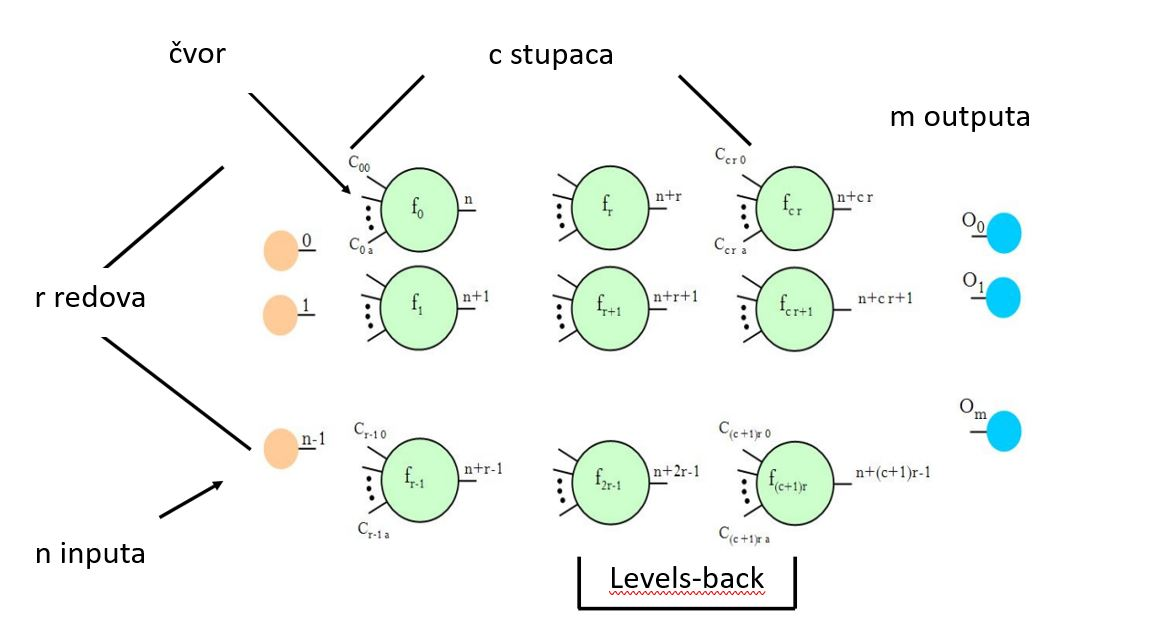
\includegraphics[width=0.9\linewidth]{cgp_mreza}
	\caption{CGP mreža \cite{CGPpresentation}}
\end{figure}  
\par 
Ovisno o broju stupaca i redova koje zadamo možemo imati različite oblike mreža. Možemo imati široke i plitke mreže (Slika 4.2 (a)), možemo imati uske i duboke mreže (Slika 4.2 (b)) ili možemo imati jednostavnu "kvadratnu" mrežu s jednakim brojem stupaca i redova.
\begin{figure}[h]
	\begin{subfigure}{0.5\textwidth}
		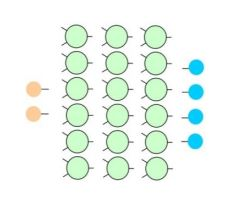
\includegraphics[width=0.9\linewidth]{cgp_wide} 
		\caption{Široka i plitka mreža \cite{CGPpresentation}}
	\end{subfigure}
	\begin{subfigure}[b]{0.5\textwidth}
		\raisebox{1.25cm}{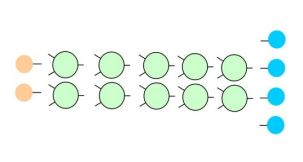
\includegraphics[width=0.9\linewidth]{cgp_deep}}
		\caption{Uska i duboka mreža \cite{CGPpresentation}}
	\end{subfigure}
	
	\caption{Mogući oblici CGP mreža}
\end{figure}
\newpage
\par Oblik i veličina mreže trebali bi biti prilagođeni zadatku s obzirom na to da premala ili prevelika mreža mogu biti izvor problema ili slabog treniranja programa. Jedna od preporučenih i zanimljivijih mreža je mreža s jednim redom i proizvoljnim brojem stupaca koja više nalikuje lancu. U ovom radu najviše se radilo s ovakvim oblikom mreže, a primjer oblika može se vidjeti na slici 4.3.

\begin{figure}[h]
	\centering
	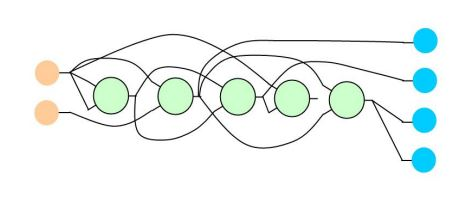
\includegraphics[width=0.9\linewidth]{cgp_chain}
	\caption{CGP mreža s jednim redom \cite{CGPpresentation}}
\end{figure}
\section{Čvorovi mreže}
\par 
 \quad Čvorovi su sastavljeni od gena koji tvore genotip, a zapravo su brojevi koji sugeriraju od kuda će čvor dobiti podatke, koje operacije će primijeniti nad podacima i od kud će doći izlazni podaci \cite{CGPbook}. 
 \par Veze između čvorova upravo su geni veza i oni nam govore iz kojeg ćemo čvora ili ulaza dobiti podatke. Broj gena veza koje sadrži svaki čvor mreže jednak je najvećem broju parametara koje traži neka od funkcija koja se može pojaviti u mreži. Pošto su svi čvorovi i ulazi numerirani ti brojevi su nam adrese. Geni veza najčešće mogu sadržavati samo adrese čvorova i ulaza iz stupaca s lijeve strane čvora za koji se adresiraju ulazni parametri, ali postoje radovi i primjeri gdje se dopuštaju ciklusi (ciklički CGP) micanjem ove restrikcije \cite{CGPbook}. Parametar \textit{\textbf{Levels-back (l)}} govori nam iz kojih stupaca s lijeve strane trenutne pozicije možemo uzeti adresu. Primjerice za \textit{l} = 1 adrese možemo uzimati samo iz lijevog neposrednog stupca. Za \textit{l} = $ n_{c} $ (l = broj stupaca) možemo dohvatiti bilo koju adresu iz mreže u bilo kojem stupcu.
 \par 
Sve funkcije koje se mogu pojaviti u čvorovima zapisane su u posebnu tablicu uz svoju brojevnu reprezentaciju. Brojevna reprezentacija postaje adresa funkcije i ona se zapisuje kao funkcijski gen koji je ključni dio svakog čvora mreže. Nakon što čvor dobije potrebne parametre preko gena veza, dohvaća se funkcija pod zadanom adresom i ona se izvršava nad danim parametrima.
\par
Izlazni geni nalaze se na krajnjoj desnoj strani mreže. Oni adresiraju čvorove ili ulaze iz kojih će se uzimati vrijednosti za konačni izlaz iz mreže. Za njih vrijede ista pravila kao i za gene veza. Na osnovu izlaza iz mreže poduzima se akcija jedinstvena za taj izlaz, čineći izlaz iz mreže odlukom mreže.\par 
Primjer mreže čvorova sa zadanim genima i vezama možemo vidjeti na slikama 4.4. i 4.5. uz funkcije u tablici 4.1.
\begin{figure}[h]
	\centering
	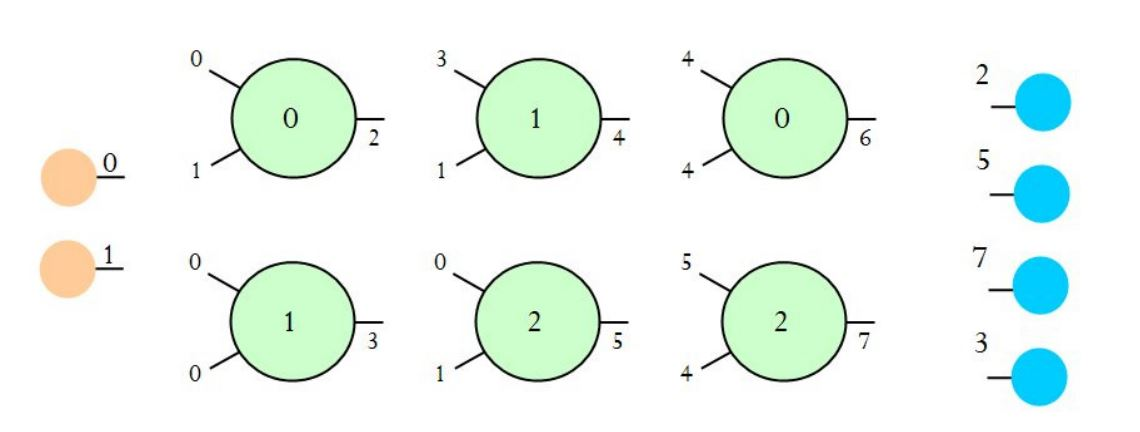
\includegraphics[width=0.9\linewidth]{cgp_mreza_zadana_a}
	\caption{CGP mreža s genima \cite{CGPpresentation}}
\end{figure}
\begin{figure}[h]
	\centering
	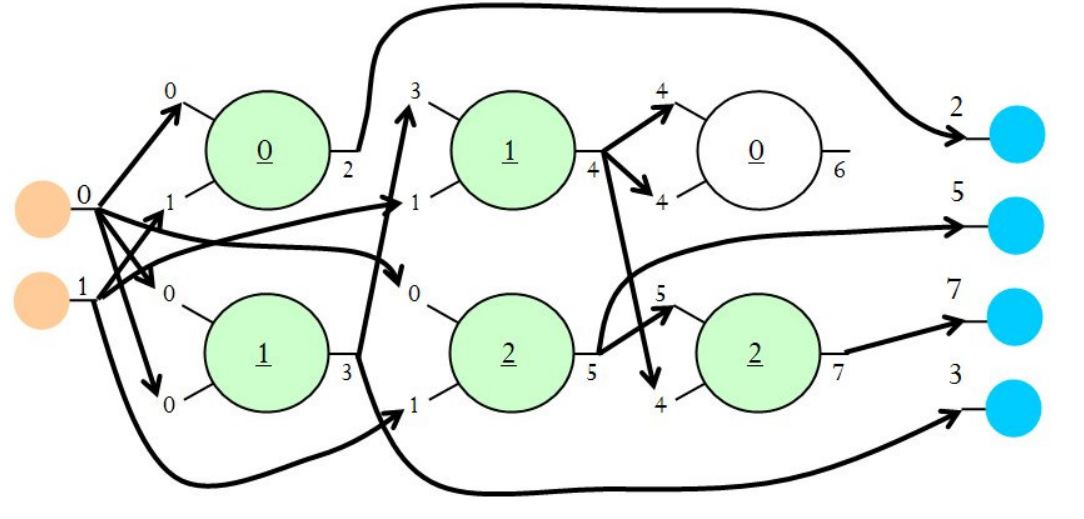
\includegraphics[width=0.9\linewidth]{cgp_mreza_zadana_b}
	\caption{CGP mreža s genima i vezama \cite{CGPpresentation}}
\end{figure}
\begin{table}[h!]
\centering
\begin{tabular}{ |c|c|c|c|  }
	\hline
	0 & 1 & 2 & 3\\
	\hline
	+ Zbroji parametre  & - Oduzmi parametre &
	* Pomnoži parametre & / Podijeli parametre\\
	\hline
\end{tabular}
\caption{Tablica funkcija (Lookup table of functions)}
\end{table}
\section{Genotip i fenotip}
\par 
\quad Pogledom na sliku 4.3. uviđamo kako je gen u trećem stupcu i prvom retku nekorišten, tj. on ne pridonosi niti jednom izlazu. On se naziva \textit{nekodirajućim genom}. Dolazimo do pojmova \textbf{genotipa} i \textbf{fenotipa}. \textit{"Dekodiranje genotipa rezultira programom koji se naziva fenotip \cite{CGPbook}."} \quad \textbf{Genotip} čine svi geni unutar mreže dok \textbf{fenotip} čine samo aktivni,\textit{ kodirajući}, geni koji utječu na izlaze iz mreže. U većim mrežama broj nekodirajućih gena može biti znatno veći od broja kodirajućih. Primjerice J. F. Miller i S. L. Smith pokazali su kako je u genotipu s 4000 čvorova postotak nekodirajućih čvorova oko 95\% \cite{geneticredundancy}. 
\par
Dekodiranje genotipa naziv je za proces kojim ćemo proći kroz genotip i utvrditi koji geni su kodirajući, a koji ne. Princip procesa je krenuti od izlaznih gena i kretati se po čvorovima čije adrese se nalaze u genima veza dok ne dođemo do ulaza u mrežu. Pseudokodom u Algoritmu 2 prikazan je proces dekodiranja.

\begin{algorithm}
	\caption{Dekodiranje genotipa}
	\begin{algorithmic}
		\State Lista čvorova
		\For{svaki izlazni gen}
		\If{adresa = adresa čvora}
		\State Označi čvor kao kodirajući
		\EndIf 
		\EndFor
		\For{svaki čvor u \textit{Lista čvorova} krenuvši od zadnjeg}
		\If{čvor je kodirajući}
		\For{gen veze u čvoru}
		\If{adresa = adresa čvora}
		\State Označi čvor kao kodirajući
		\EndIf 
		\EndFor
		\EndIf
		\EndFor\newline
		\Return Lista čvorova
	\end{algorithmic}
\end{algorithm}
\newpage
\section{CGP kao niz brojeva}
\par 
\quad Tijekom opisa Kartezijevog genetskog programiranja susreli smo se već nekoliko puta s brojevima i brojevnom reprezentacijom, a svi brojevi zapravo su adrese. Upravo zbog tih brojeva postoji vrlo jednostavan zapis genotipa i to u obliku niza brojeva. U tom nizu moramo znati raspoznati gene - funkcijski geni, geni veza i izlazni geni. Iako u nizu nećemo imati nikakvu posebnu reprezentaciju znat ćemo točno koji je gen koji ako znamo koliko parametara svaki čvor treba primiti i koliko izlaza imamo. Uzmemo li mrežu na Slici 4.4 kao primjer, možemo konstruirati reprezentaciju mreže krenemo li od gornjeg lijevog čvora: \newline

\makebox[\textwidth][c]{%
	\begin{minipage}{0.1\textwidth}
		\par \textbf{\underline{0} 0 1}
\end{minipage}}\newline
\par 
U čitanje niza ulazimo sa znanjem da je najveći broj parametara potreban nekoj od mogućih funkcija dva te da imamo dva izlaza iz mreže. Slijeva nadesno imamo: funkcijski gen s brojem \textit{0} koji adresira funkciju zbrajanja u tablici funkcija (Tablica 4.1), prvi gen veze koji adresira od kud dobivamo prvi parametar što bi u ovom primjeru bio \textit{0} - prvi ulaz/input, drugi gen veze koji adresira od kud dobivamo drugi parametar što bi u ovom primjeru bio \textit{1} - drugi ulaz/input. Nastavimo li dalje prolaziti po čvorovima dobivamo sljedeći niz: \newline

\makebox[\textwidth][c]{%
	\begin{minipage}{0.7\textwidth}
		\par \textbf{\underline{0} 0 1  \quad\underline{1} 0 0  \quad\underline{1} 3 1  \quad\underline{2} 0 1  \quad\underline{0} 4 4  \quad\underline{2} 5 4  \qquad 2 5 7 3}
\end{minipage}}\newline
\par
Pogledamo li u nizu treći čvor vidimo kako njegov prvi gen veze sadrži broj \textit{3}. Pošto imamo samo dva ulaza i njihove adrese su \textit{0} i \textit{1} to znači kako je adresiran jedan od čvorova; u ovom slučaju drugi čvor u prvom stupcu. Prema tome, adrese čvorova nastavljaju se na adrese ulaza jer oni sami postaju ulazi za neki sljedeći čvor ili izlaz. Adrese se povećavaju s lijeva nadesno i od vrha stupca prema dnu stupca.\par
Zadnji dio niza koji je ovdje posebno odvojen od ostatka niza čine izlazni geni. U ovom slučaju na izlaz iz mreže spojeni su prvi, drugi, četvrti i šesti čvor. \par
Ovakav oblik CGP mreže/programa izuzetno je koristan i pojednostavljuje inicijalizaciju, izvršavanje i promjenu programa. Promjene nad populacijom i pojedinim programima obrađuju se kasnije u zasebnim poglavljima.\par 

\section{Inicijalizacija programa/populacije}
 \quad Inicijalizacija, kao i u običnom genetskom programiranju, podrazumijeva stvaranje nasumične populacije programa. U ovom slučaju to bi bili nizovi nasumičnih brojeva. \par 
 Iako brojevi jesu nasumični, postoje pravila koja smo ranije postavili i koja moramo poštivati. Nizovi moraju biti smisleni i slijediti formu sličnoj onoj iz primjera gdje znamo na kojim mjestima se nalaze funkcijski geni, na kojima geni veza i na kojima izlazni geni. Osim forme, adrese koje se mogu pojaviti na određenim pozicijama moraju biti ograničene na isti način kao u mreži. Funkcijski geni smiju imati samo adrese iz tablice funkcija, ali te adrese mogu se pojaviti u bilo kojem dijelu niza gdje se nalaze funkcijski geni. Geni veza (osim ako se radi o cikličkom CGP-u) smiju imati samo adrese čvorova iz stupaca lijevo od njihovog stupca, naravno s danim ograničenjem Levels-back. Informaciju o tome u kojem se stupcu nalazi koji čvor dobivamo iz kombinacije informacija: broj redova mreže, tj. koliko čvorova imamo u svakom stupcu, i praćenjem rednog broja čvora u kojem se nalazimo. Izlazni geni smiju sadržavati adrese svih čvorova i ulaza u mreži.  \par 
 Slijedeći ova pravila možemo inicijalizirati cijelu populaciju programa jednostavnog zapisa u kratkom roku.\newpage \par U nastavku možemo vidjeti jednu takvu populaciju mreža koje imaju šesnaest ulaza, četiri izlaza, širinu jedan, dubinu osam i maksimalan broj parametara funkcija dva. Radi preglednosti nizovi su podijeljeni na čvorove i izlaze, funkcijski geni su \underline{podcrtani}, a izlazni geni su \textbf{podebljani}.\newline
 
\begin{table}[h!]
\centering
\begin{tabular}{ |c|c|c|c|c|c|c|c|c|  }
	\hline
	\underline{4} 6 14 & \underline{5} 15 16 & \underline{4} 0 8 & \underline{4} 15 15 & \underline{2} 8 3 & \underline{4} 7 10 & \underline{1} 17 3 & \underline{3} 13 3 & \textbf{13 23 4 10}\\
	\hline
\end{tabular}
\end{table}

\begin{table}[h!]
	\centering
	\begin{tabular}{ |c|c|c|c|c|c|c|c|c|  }
		\hline
	 \underline{4} 14 5 & \underline{3} 15 6 & \underline{5} 1 7 & \underline{4} 7 12 & \underline{2} 0 15 & \underline{1} 19 3 & \underline{1} 16 9 & \underline{0} 14 3 & \textbf{20 22 1 11} \\
		\hline
	\end{tabular}
\end{table}

\begin{table}[h!]
	\centering
	\begin{tabular}{ |c|c|c|c|c|c|c|c|c|  }
		\hline
		\underline{4} 14 7 & \underline{3} 1 4 & \underline{5} 13 11 & \underline{1} 15 1 & \underline{2} 6 2 & \underline{4} 12 9 & \underline{1} 1 13 & \underline{5} 12 3 & \textbf{7 23 20 20}\\
		\hline
	\end{tabular}
\end{table}

\begin{table}[h!]
	\centering
	\begin{tabular}{ |c|c|c|c|c|c|c|c|c|  }
		\hline
		\underline{2} 15 8 & \underline{1} 2 7 & \underline{2} 17 9 & \underline{1} 4 15 & \underline{3} 8 1 & \underline{5} 6 18 & \underline{2} 19 10 & \underline{3} 14 19 & \textbf{0 5 10 21}\\
		\hline
	\end{tabular}
\end{table}

  
 
\section{Izvođenje programa}  
\quad Sad kad smo upoznati s oblikom programa i pojmom fenotipa možemo govoriti o izvođenju programa. Prije izvođenja programa potrebno ga je dekodirati kako bi radili samo s onim čvorovima koji nam utječu na izlaz iz mreže. Nakon što smo dobili fenotip, počinjemo s procesom koji je po prolazu kroz mrežu obrnut od dekodiranja. Pod pretpostavkom da radimo s necikličnom mrežom, imamo unaprijednu (eng. feed-forward) mrežu koja obrađuje i propagira podatke od ulaza prema izlazu. Izvođenje programa se zbog toga odvija stupac po stupac od ulaza prema izlazu kako ni u jednom trenutku ne bi došli do čvora koji ima nedefinirane ulazne parametre. Za svaki čvor slijedimo njegove gene veza do parametara koje uvrštavamo u funkciju adresiranu u funkcijskom genu. Rezultat funkcije zapamtimo kao izlaz iz čvora. Nastavljamo dalje čvor po čvor dok ne dođemo do izlaznih gena koji dohvaćaju izlaze čvorova ili ulaze u mrežu. \par
Ovime smo pokrenuli i izvršili program koji smo sastavili. Kao rezultat izvođenja programa dobili smo izlaz koji se može interpretirati kao odgovor na zadani zadatak ili dalje koristiti u svrhu rješavanja zadatka.